\subsection{Other paradoxes and fallacies}

Data ellipses can also be used to visualize and understand other paradoxes and
fallacies that occur with linear models.  We consider situations in which there
is a principal relationship between variables $y$ and $x$ of interest, but (as in the preceding subsection) the data
are stratified in $g$  samples by a factor (``group'') that might correspond
to different subpopulations (e.g., men and women, age groups),
different spatial regions (e.g., states), different points in time, or some
combination of the above.

In some cases, group may be unknown, or may not have been included in the model,
so we can only estimate the marginal association between $y$ and $x$,
giving a slope $\beta_{\textrm{marginal}}$ and correlation $r_{\textrm{marginal}}$.
In other cases, we may not have individual data, but only aggregate group
data, $(\bar{y}_i, \bar{x}_i), i=1, \dots , g$, from which we can estimate
the between-groups (``ecological'') association, with slope
$\beta_{\textrm{between}}$ and correlation $r_{\textrm{between}}$.
When all data are available and the model is an ANCOVA model of the form
$y \sim x + \textrm{group}$,
we can estimate a common conditional, within-group slope,
$\beta_{\textrm{within}}$, or, with the model $y \sim x + x \times \textrm{group}$,
the separate within-group slopes, $\beta_i$.


\begin{figure}[htb]
 \begin{minipage}[b]{.49\linewidth}
  \centering
  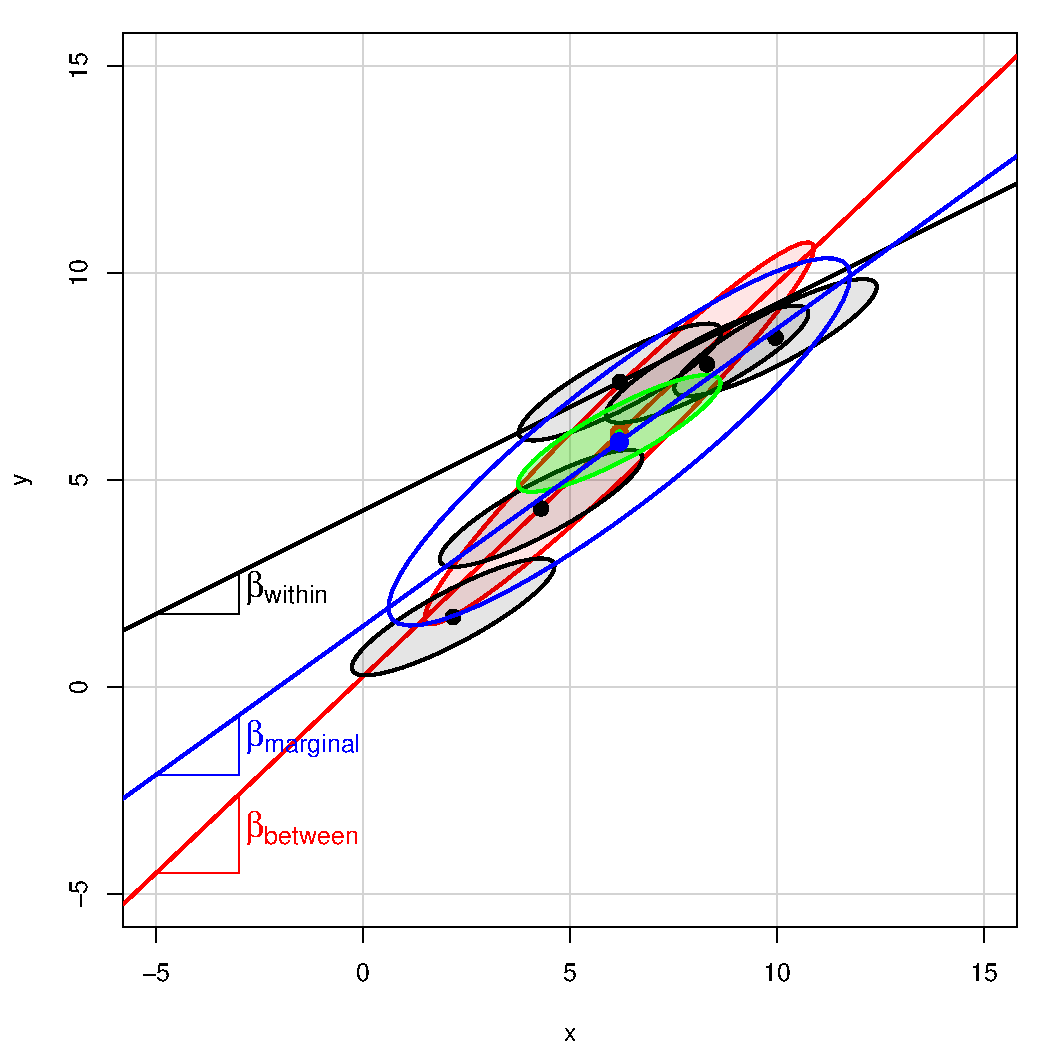
\includegraphics[width=1\linewidth]{fig/between-within1}
 \end{minipage}%
 \hfill
 \begin{minipage}[b]{.49\linewidth}
  \centering
  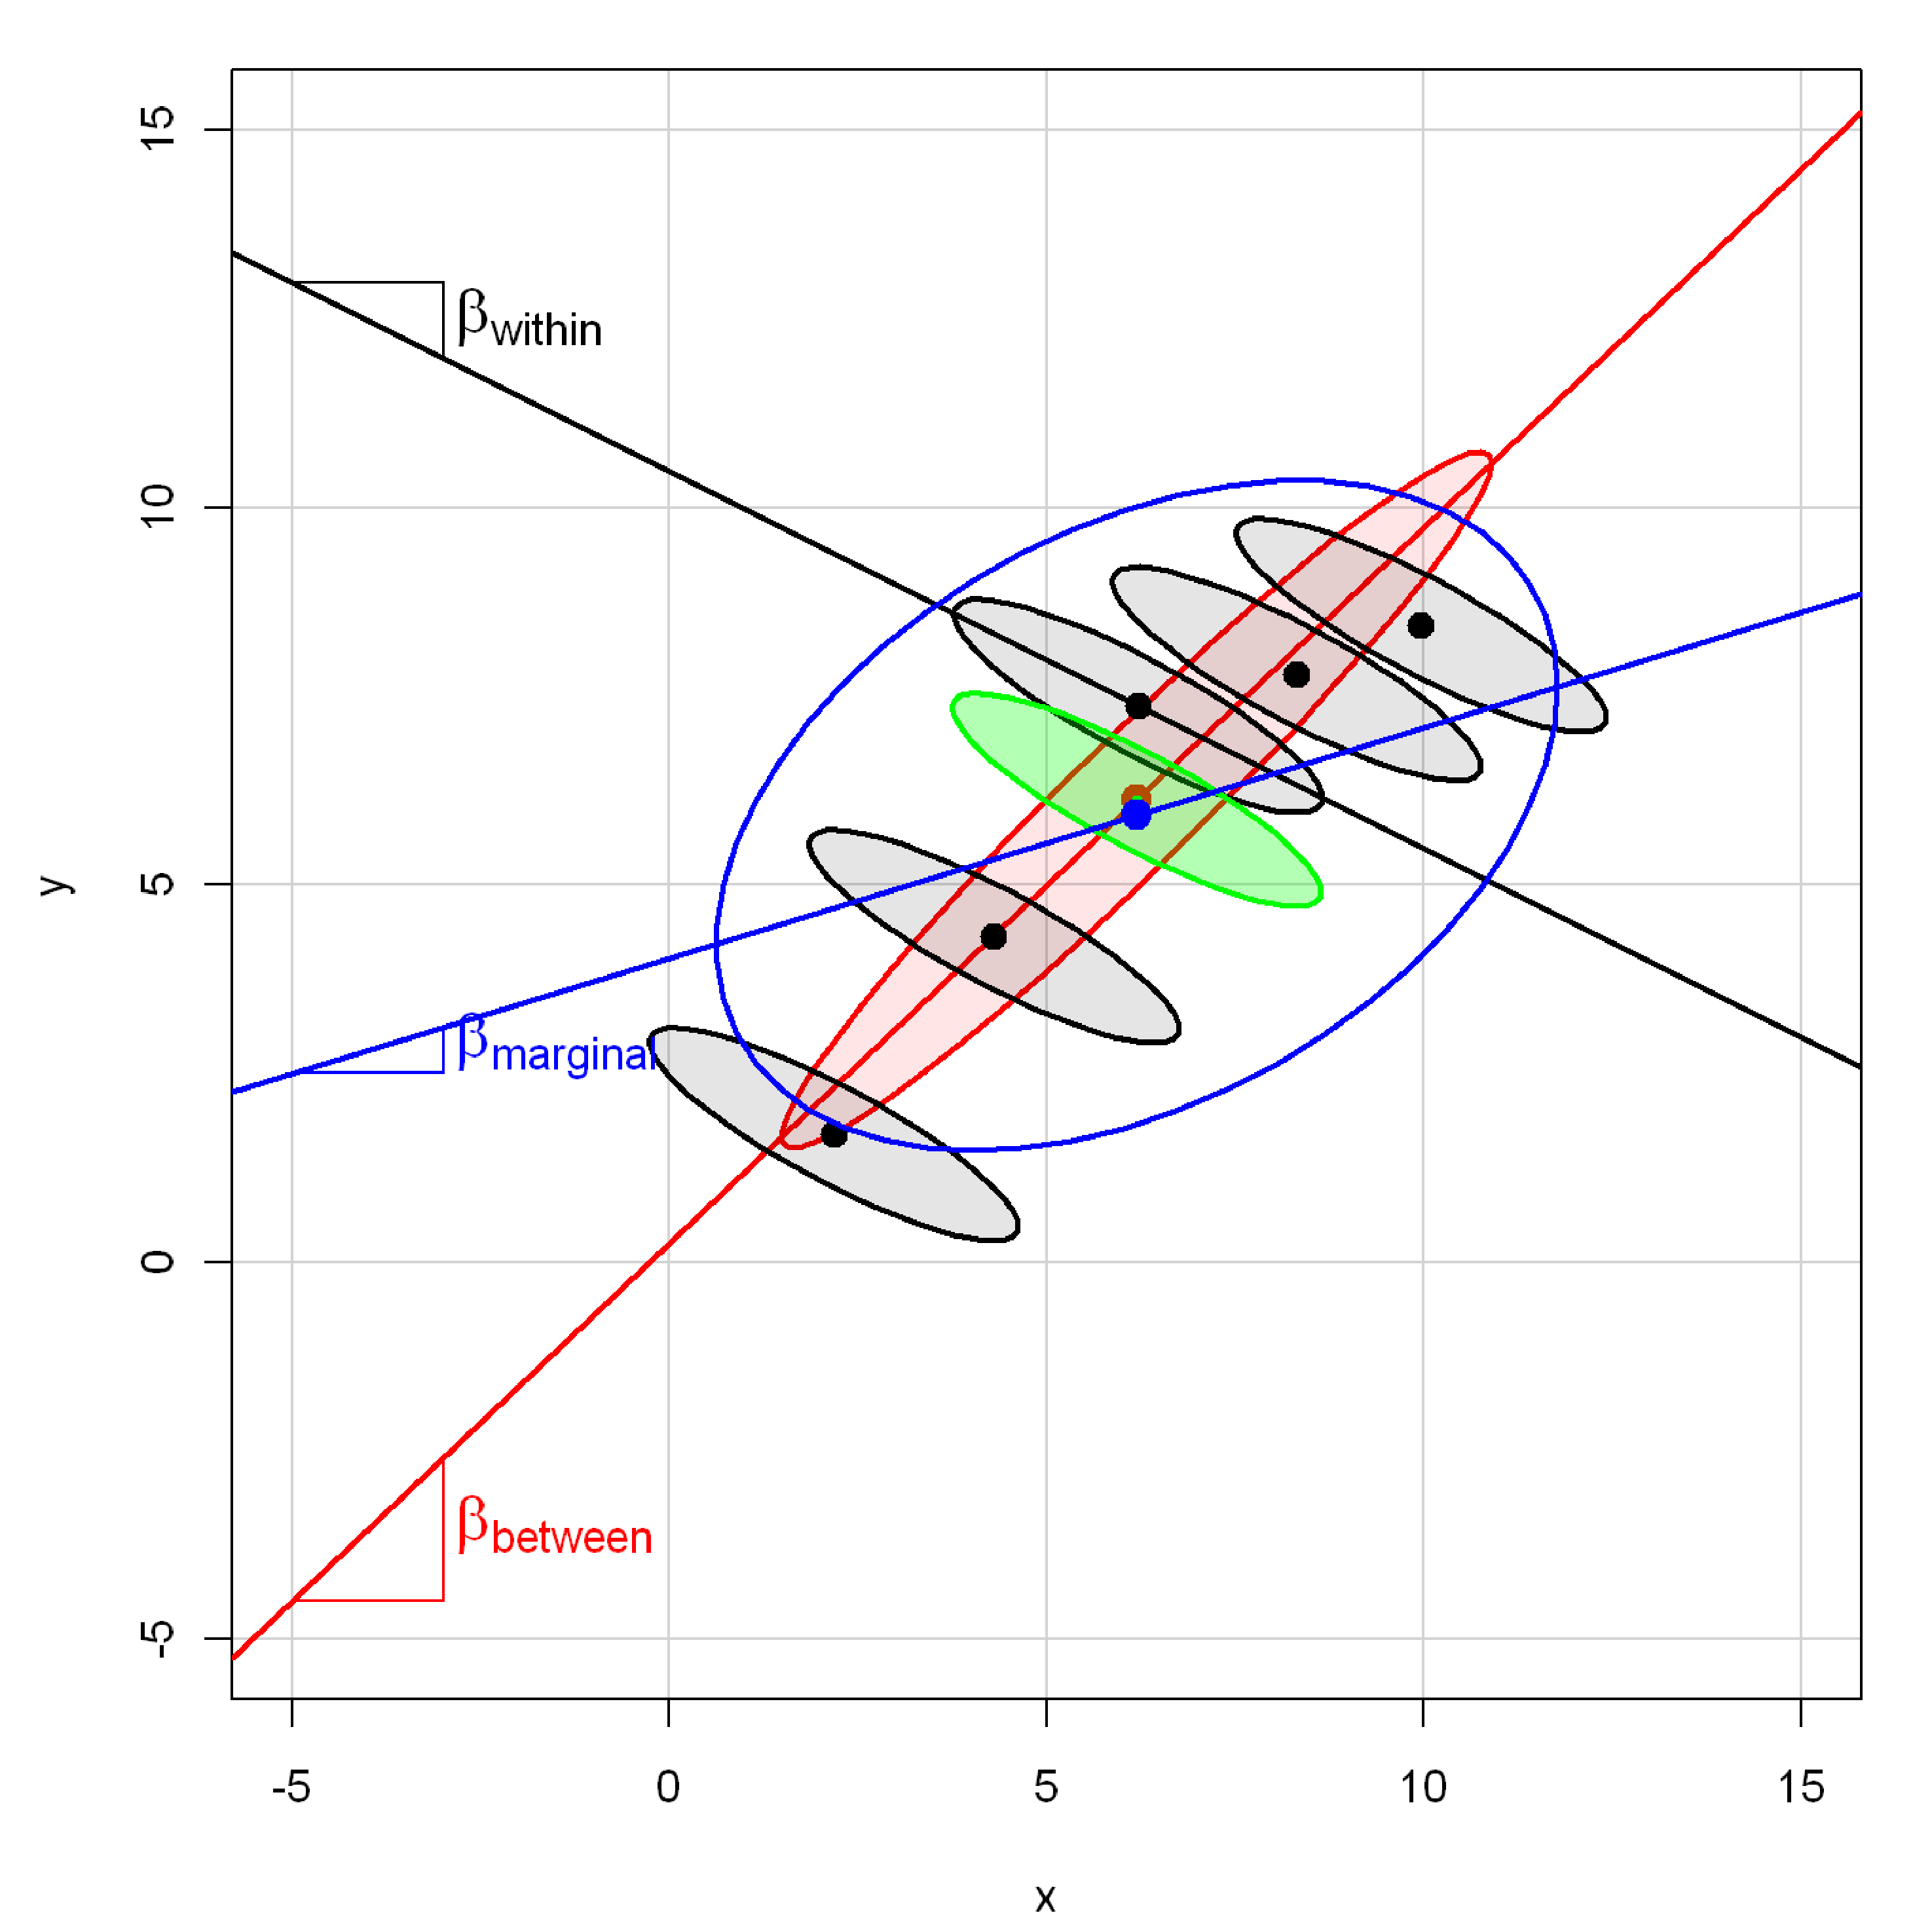
\includegraphics[width=1\linewidth]{fig/between-within2}
 \end{minipage}
  \caption{Paradoxes and fallacies: between (ecological), within (conditional) and whole-sample (marginal) associations.
  In both panels, the five groups have the same group means, and $\Var(x)=6$ and $\Var(y)=2$ within each group.
  The within-group correlation is $r = +0.87$ in all groups in the left panel, and is $r = -0.87$ in the right panel.
  The green ellipse shows the average within-group data ellipse.}
  \label{fig:between-within}
\end{figure}

\figref{fig:between-within} illustrates these estimates in a simulation of five groups, with $n_i=10$,  means
$\bar{x}_i = 2 \, i + \mathcal{U}(-0.4, 0.4)$  and
$\bar{y}_i = \bar{x}_i + \mathcal{N}(0, 0.5^2)$, 
so that $r_{\textrm{between}} \approx 0.95$.
Here $\mathcal{U}(a,b)$ represents the uniform distribution between $a$ and $b$, and
$\mathcal{N}(\mu,\sigma^2)$ represents the normal distribution with mean $\mu$ and 
variance $\sigma^2$.
For simplicity, we have set the within-group covariance matrices to be identical in all groups, with
$\Var(x)=6$, $\Var(y)=2$ ,and $\Cov(x,y)=\pm 3$ in the left and right panels, respectively, giving
$r_{\textrm{within}} = \pm 0.87$.

In the left panel, the conditional, within-group slope is smaller than the ecological, between-group slope,
reflecting the smaller within-group than between-group correlation.
In general, however, it can be shown that
\begin{equation*}
\vec{\beta}_{\textrm{marginal}} \in [\vec{\beta}_{\textrm{within}} , \vec{\beta}_{\textrm{between}} ] \comma
\end{equation*}
which is also evident in the right panel, where the within-group slope is negative.
This result follows from the fact that the marginal data ellipse for the total sample
has a shape that is a convex combination (weighted average) of the average within-group
covariance of $(x, y)$, shown by the green ellipse in  \figref{fig:between-within},
and the  covariance of the means $(\bar{x}_i, \bar{y}_i)$, shown by the red between-group ellipse.
In fact, the between and within data ellipses in  \figref{fig:between-within}
are just (a scaling of) the $\mat{H}$ and $\mat{E}$ ellipses in an hypothesis-error (HE) plot for the
MANOVA model, $(x, y) \sim \textrm{group}$, as will be developed in \secref{sec:mlm}.
See \figref{fig:between-HE} for a visual demonstration, using the same data  as in   \figref{fig:between-within}.
%\TODO{Can we show this analytically in some insightful way?}

\begin{figure}[htb]
 \begin{minipage}[b]{.49\linewidth}
  \centering
  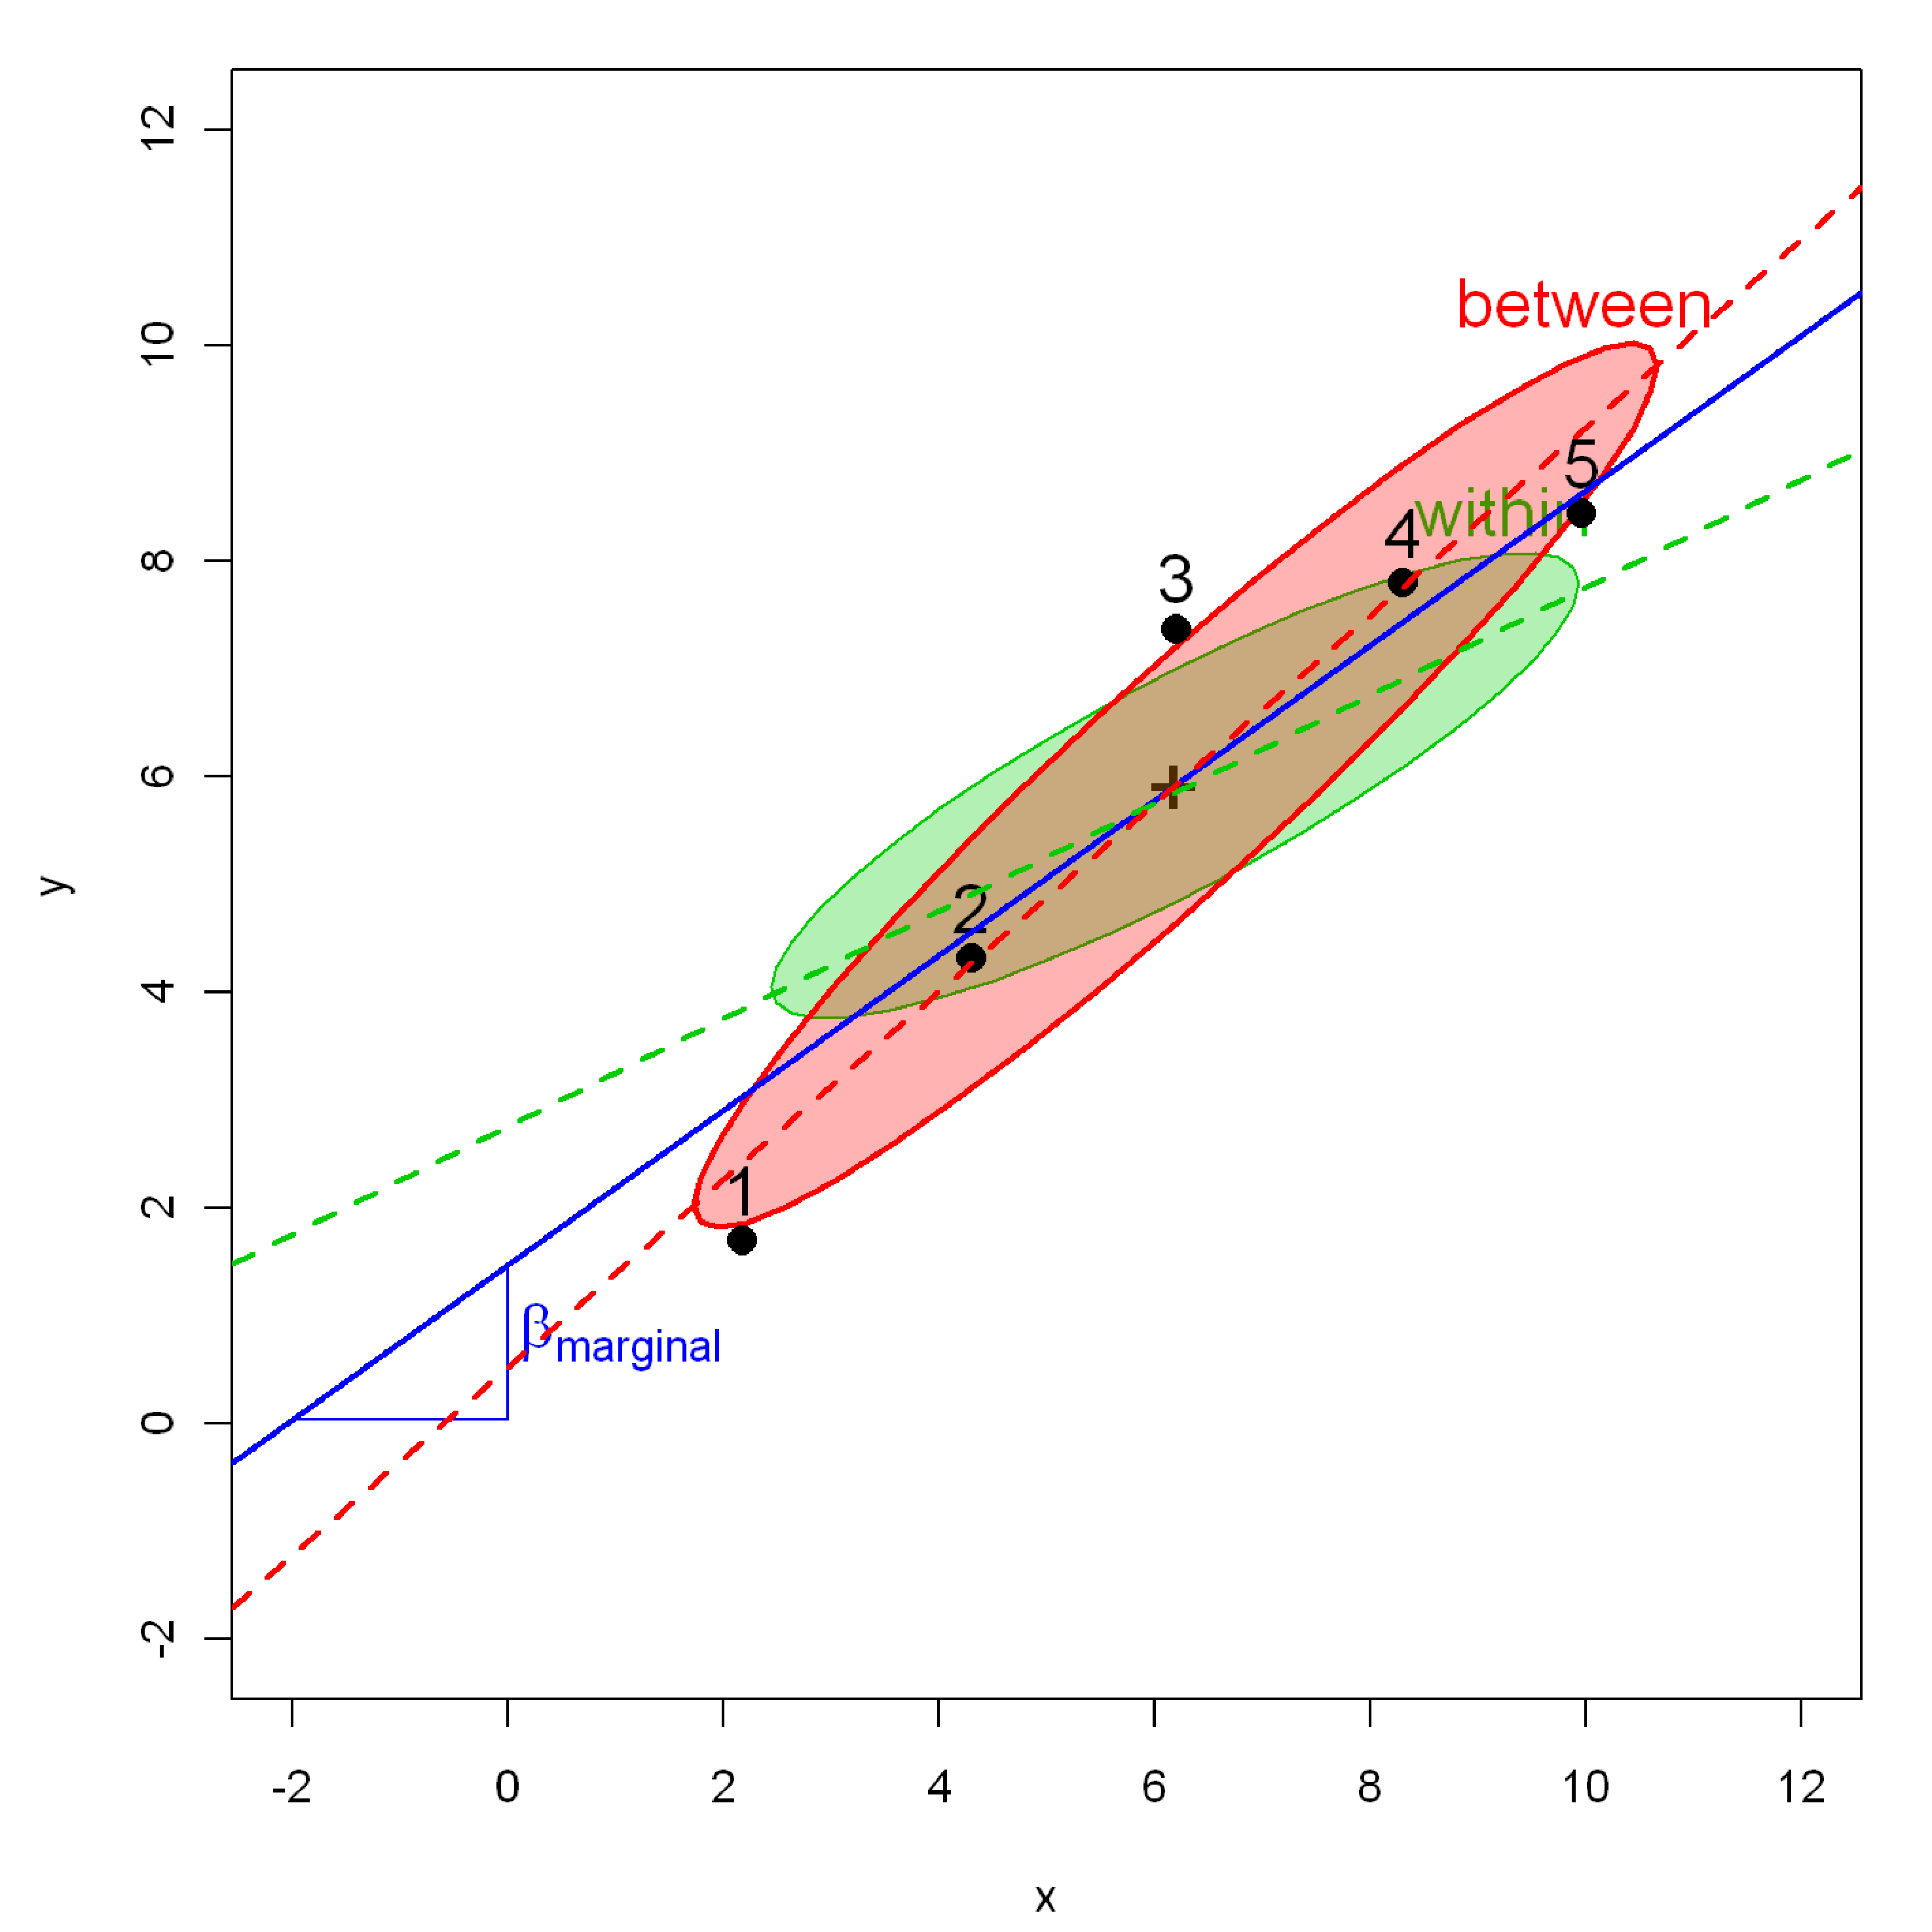
\includegraphics[width=1\linewidth]{fig/between-HE1}
 \end{minipage}%
 \hfill
 \begin{minipage}[b]{.49\linewidth}
  \centering
  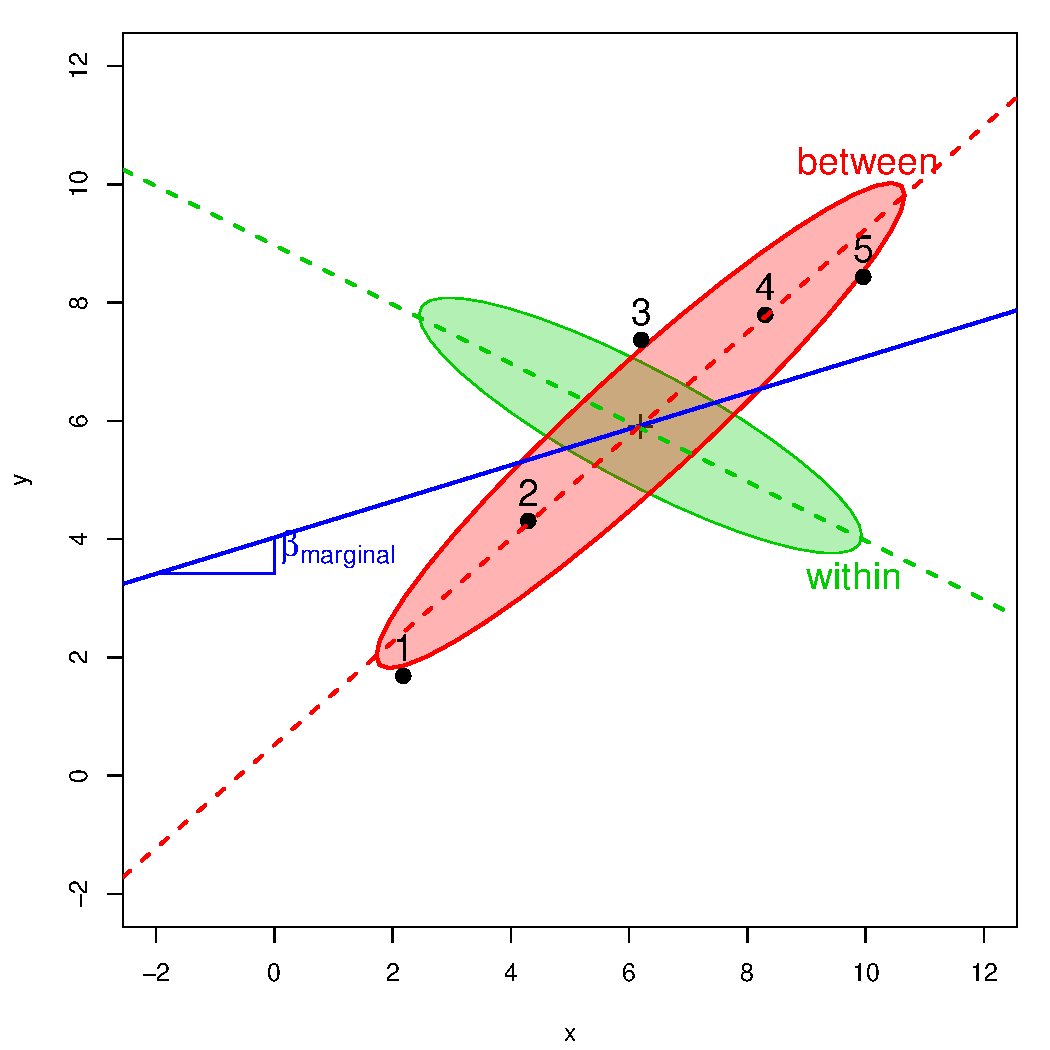
\includegraphics[width=1\linewidth]{fig/between-HE2}
 \end{minipage}
  \caption{Visual demonstration that $\vec{\beta}_{\textrm{marginal}}$ lies between $\vec{\beta}_{\textrm{within}}$ and $\vec{\beta}_{\textrm{between}}$.
  Each panel shows an HE plot for the MANOVA model $(x, y) \sim \textrm{group}$, in which the within and between ellipses are identical to
  those in \figref{fig:between-within}, except for scale.}
  \label{fig:between-HE}
\end{figure}

The right panels of \figref{fig:between-within} and \figref{fig:between-HE} 
provide a prototypical illustration of Simpson's paradox,
where $\beta_{\textrm{within}}$ and $\beta_{\textrm{marginal}}$ can have opposite signs. Underlying this is a
more general \emph{marginal fallacy} (requiring only substantively different estimates, but not necessarily
different signs),
that can occur when some important factor or covariate is unmeasured
or has been ignored. The fallacy consists of estimating the unconditional or marginal
relationship ($\beta_{\textrm{marginal}}$) and believing that it reflects the conditional relationship, or that
those pesky ``other'' variables will somehow average out. In practice, the marginal fallacy probably occurs most
often when one views a scatterplot matrix of $(y, x_1, x_2, \dots)$ and believes that the slopes of
relationships in the separate panels reflect the pairwise conditional relationships with other variables
controlled. In a regression context, the antidote to the marginal fallacy is the added-variable
plot (described in \secref{sec:avp}),
which displays the conditional relationship between the response and a predictor directly, controlling for all other predictors.

The right panels of \figref{fig:between-within} and \figref{fig:between-HE} also illustrate Robinson's paradox \citep{Robinson:1950},
where $\beta_{\textrm{within}}$ and $\beta_{\textrm{between}}$ can have opposite signs.%
\footnote{
William Robinson \citeyearpar{Robinson:1950} examined the relationship between literacy rate and percentage
of foreign-born immigrants in the U.S. states from the 1930 Census.
He showed that there was a surprising
positive correlation, $r_{\textrm{between}}= 0.526$ at the state level,
suggesting that foreign birth was associated with greater literacy;
at the individual level, the correlation $r_{\textrm{within}}$ was $-0.118$, suggesting the opposite.
An explanation for the paradox was that immigrants tended to settle in regions of greater than
average literacy.
}
The more general \emph{ecological fallacy} (e.g., \citealp{Lichtman:1974,Kramer:1983})
is to draw conclusions from aggregated data, estimating
$\beta_{\textrm{between}}$ or $r_{\textrm{between}}$, believing that they reflect relationships
at the individual level, estimating $\beta_{\textrm{within}}$ or $r_{\textrm{within}}$.
Perhaps the earliest instance of this was Andr\'e-Michel Guerry's \citeyearpar{Guerry:1833} use of thematic maps of
France depicting rates of literacy, crime, suicide, and other ``moral statistics'' by department to argue
about the relationships of these moral variables as if they reflected individual behavior.%
\footnote{
Guerry was certainly aware of the logical problem of ecological inference, at least in general terms
\citep{Friendly:07:guerry}, and carried out several side-analyses to examine potential confounding
variables.
}
As can be seen in \figref{fig:between-within}, the ecological fallacy can often be resolved
by accounting for some confounding variable(s) that vary between groups.

Finally, there are situations where only a subset of the relevant data are available (e.g.,
one group in \figref{fig:between-within}), or when the relevant data are available only
at the individual level,
so that only the conditional relationship,
$\beta_{\textrm{within}}$ can be estimated. The \emph{atomistic fallacy}
(also called the \emph{fallacy of composition} or the
\emph{individualistic fallacy}), e.g., \citet{Alker:1969,Riley:1963},
is the inverse to the
ecological fallacy, and consists of believing that one can draw conclusions
about the ecological relationship, $\beta_{\textrm{between}}$, from the conditional one.

The atomistic fallacy occurs most often in the context of multilevel models \citep{Diez-Roux:1998}
where it is desired to draw inferences regarding variability of higher-level units
(states, countries) from data collected from lower-level units.
For example, imagine that the right panel of \figref{fig:between-within} depicts the negative
relationship of mortality from heart disease ($y$) with individual income ($x$) for
individuals within countries. It would be fallacious to infer that the same slope
(or even its sign) applies to a between-country analysis of heart disease mortality vs.
GNP per capita. A positive value of $\beta_{\textrm{between}}$ in this context might
result from the fact that, across countries, higher GNP per capita is associated with
less healthy diet (more fast food, red meat, larger portions), leading to increased heart disease.

